\documentclass[12pt,a4paper]{article}
\usepackage[utf8]{inputenc}
\usepackage[german]{babel}
\usepackage[T1]{fontenc}
\usepackage{amsmath}
\usepackage{amsfonts}
\usepackage{amssymb}
\usepackage{graphicx}
\usepackage[left=2.5cm,right=2.5cm,top=2cm,bottom=2cm]{geometry}
\author{Gruppe C14 \\ Julián Häck, Martin Koytek, Lars Wenning, Erik Zimmermann}
\usepackage{multicol}
\usepackage{float}
\usepackage{subfigure}
\begin{document}
\section{Rauschmessung}
Als Vorversuch  zur Messung der Dampfdruckkurve muss zunächst das Rauschen der Temperatursensoren und der Drucksensoren vermessen werden. Das Rauschen pflanzt sich als statistischer Fehler auf die Hauptmessung fort.
Dazu wurden in Cassy folgende Messwerterfassungseinstellungen vorgenommen:
\begin{table}[H]\centering
\caption{Messparameter}
\begin{tabular}{c|cc}
 & Gruppe 1 & Gruppe 2 \\ 
 \hline
Intervall & 50ms & 20ms \\ 
Anzahl & 2000 & 5000 \\ 
Messzeit & 100s & 100s \\ 
\end{tabular} 
\end{table}


\subsection{Rauschmessung der Temperatursensoren}
Die Temperatur wurde bei möglichst konstanter Temperatur und konstantem Druck gemessen. Die so ermittelten Temperaturschwankungen sind folglich hauptsächlich auf ein Rauschen der Sensoren zurückzuführen. 
Beide Gruppen haben eine Rauschmessung bei Zimmertemperatur im abgeschlossenen Behälter durchgeführt.


\begin{figure}[H]
    \subfigure[Gruppe 1]{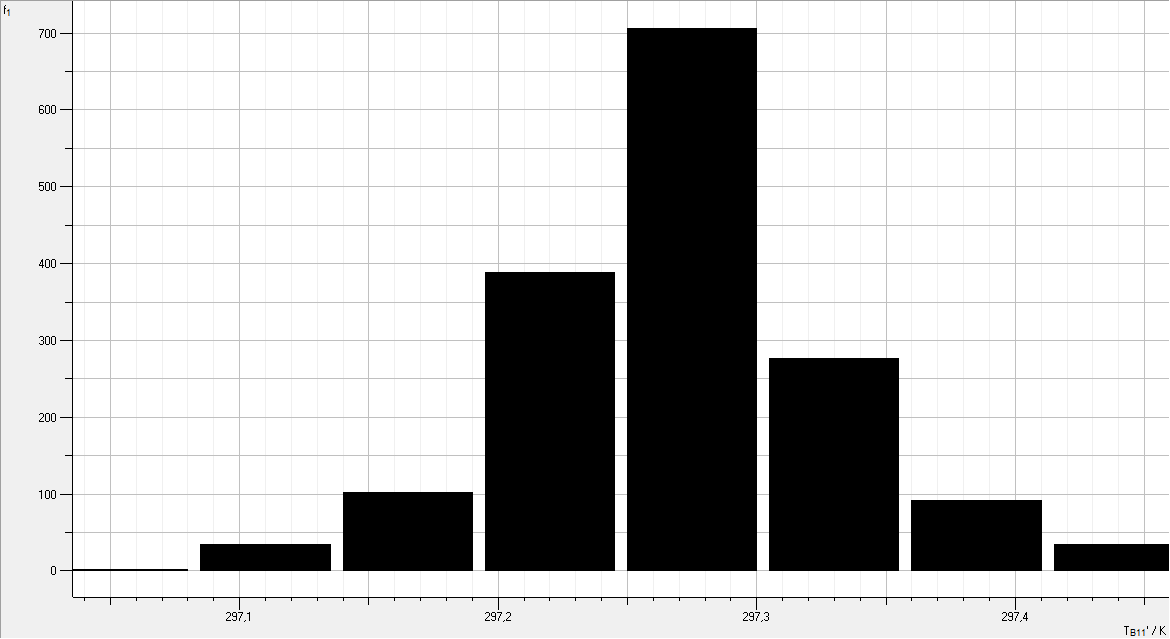
\includegraphics[width=0.49\textwidth]{Bilder/Zimmertemperatur_G1_1.png}}
    \subfigure[Gruppe 2]{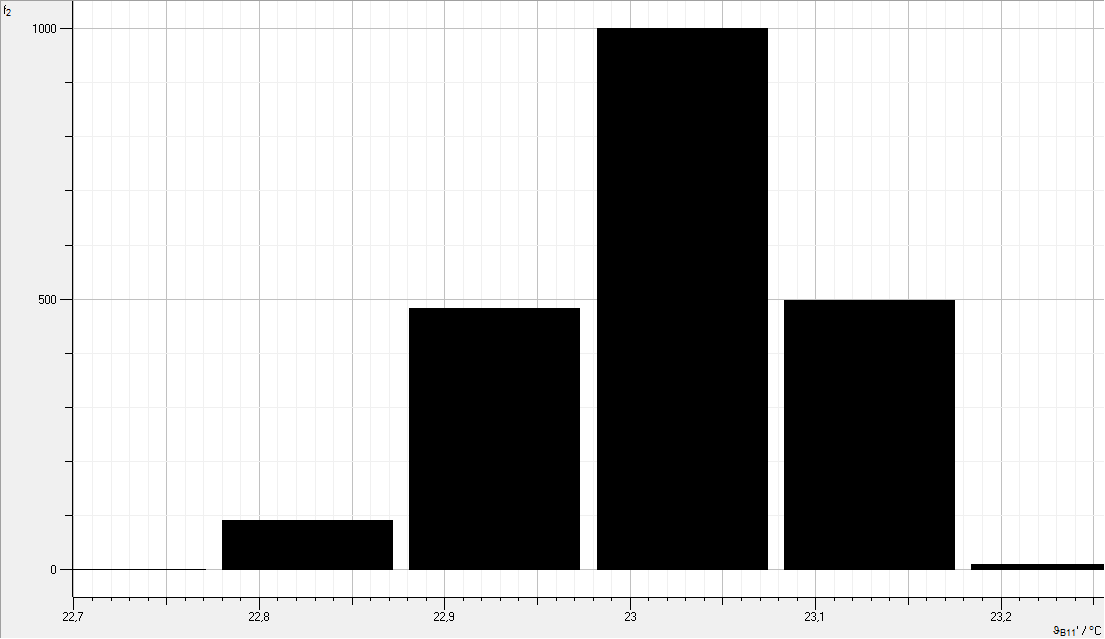
\includegraphics[width=0.49\textwidth]{Bilder/Zimmertemperatur_G2.png}}
\caption{Rauschmessung der Temperatur bei Zimmertemperatur}
\end{figure}

\begin{table}[H]\centering
\caption{Rauschmessung der Temperatur bei Zimmertemperatur}
\begin{tabular}{c|c|c}
 & Gruppe 1 & Gruppe 2 \\ 
\hline 
$T_M$ in K & 297.26 & 296.17 \\ 
$\sigma_T$ in K & 0.054 & 0.069 \\  
\end{tabular} 
\end{table}

Diese Fehler auf die Einzelwerte der Temperatur wurden später als statistische Fehler bei der Hauptmessung verwendet.
\subsection{Rauschmessung der Drucksensoren}
Die Rauschmessung der Drucksensoren wurde jeweils simultan mit der Rauschmessung der Temperatursensoren durchgeführt.


\begin{figure}[H]
    \subfigure[Gruppe 1]{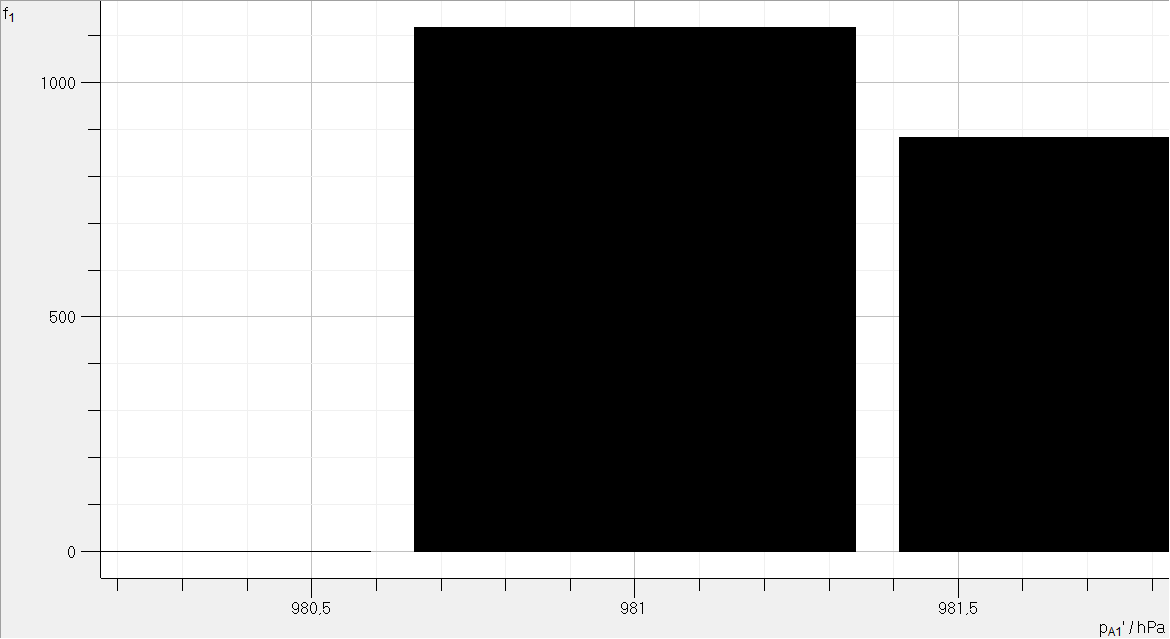
\includegraphics[width=0.49\textwidth]{Bilder/Zimmertemperatur_Druck_G1_1.png}}
    \subfigure[Gruppe 2]{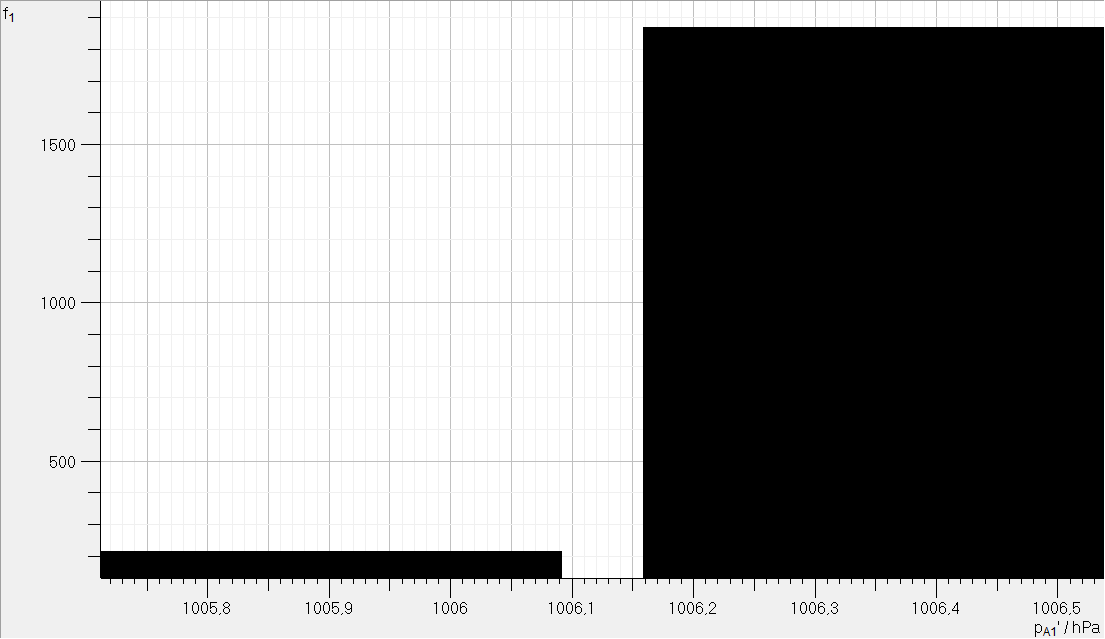
\includegraphics[width=0.49\textwidth]{Bilder/Zimmertemperatur_Druck_G2.png}}
\caption{Rauschmessung des Drucks bei Zimmertemperatur}
\end{figure}

\begin{table}[H]\centering
\caption{Rauschmessung des Drucks bei Zimmertemperatur}
\begin{tabular}{c|c|c}
 & Gruppe 1 & Gruppe 2 \\ 
\hline 
$P_M$ in hPa & 981.443 & 1006.265 \\ 
$\sigma_P$ in hPa & 0.370 & 0.348 \\  
\end{tabular} 
\end{table}

Diese Fehler auf die Einzelwerte des Drucks wurden später als statistische Fehler bei der Hauptmessung und bei der Vermessung der Dichtigkeit verwendet.

\end{document}